\documentclass[11pt]{article}
\usepackage[a4paper, margin=1in]{geometry}
\usepackage{graphicx}
\usepackage{float}
\usepackage{amsmath}
\usepackage{booktabs}
\usepackage{caption}
\usepackage{hyperref}

\title{\textbf{Life Expectancy Analysis Using Regression and Statistical Testing}}
\author{Machine Learning Assignment 1 – Part 2}
\date{}

\begin{document}

\maketitle

\section*{Abstract}
This study analyzes life expectancy data provided by the World Health Organization (WHO) to understand the impact of socioeconomic and health indicators on life expectancy. We perform data preprocessing, statistical hypothesis testing, correlation analysis, and regression modeling to explore insights into country-level life expectancy outcomes. The analysis includes both models with and without country-specific information.

\section{Introduction}
Life expectancy is a crucial indicator of a country's overall development and healthcare quality. This project aims to identify and evaluate key factors affecting life expectancy by using a dataset from WHO. We analyze patterns in health indicators, test hypotheses about group differences, compute correlations, and build predictive models to extract meaningful relationships.

\section{Data Cleaning and Preprocessing}
The dataset contains records from various countries over multiple years. We handled missing values by:
\begin{itemize}
    \item Using median imputation for numerical variables.
    \item Dropping rows with excessive missingness.
\end{itemize}

Categorical variables like \texttt{Status} (Developed vs Developing) were encoded using binary values. We standardized numerical features to improve model performance and comparability across variables.

\section{Exploratory Data Analysis}

\subsection{Boxplot Distribution of Features}
To detect variability and outliers across features, we generated a boxplot of all normalized variables.

\begin{figure}[H]
    \centering
    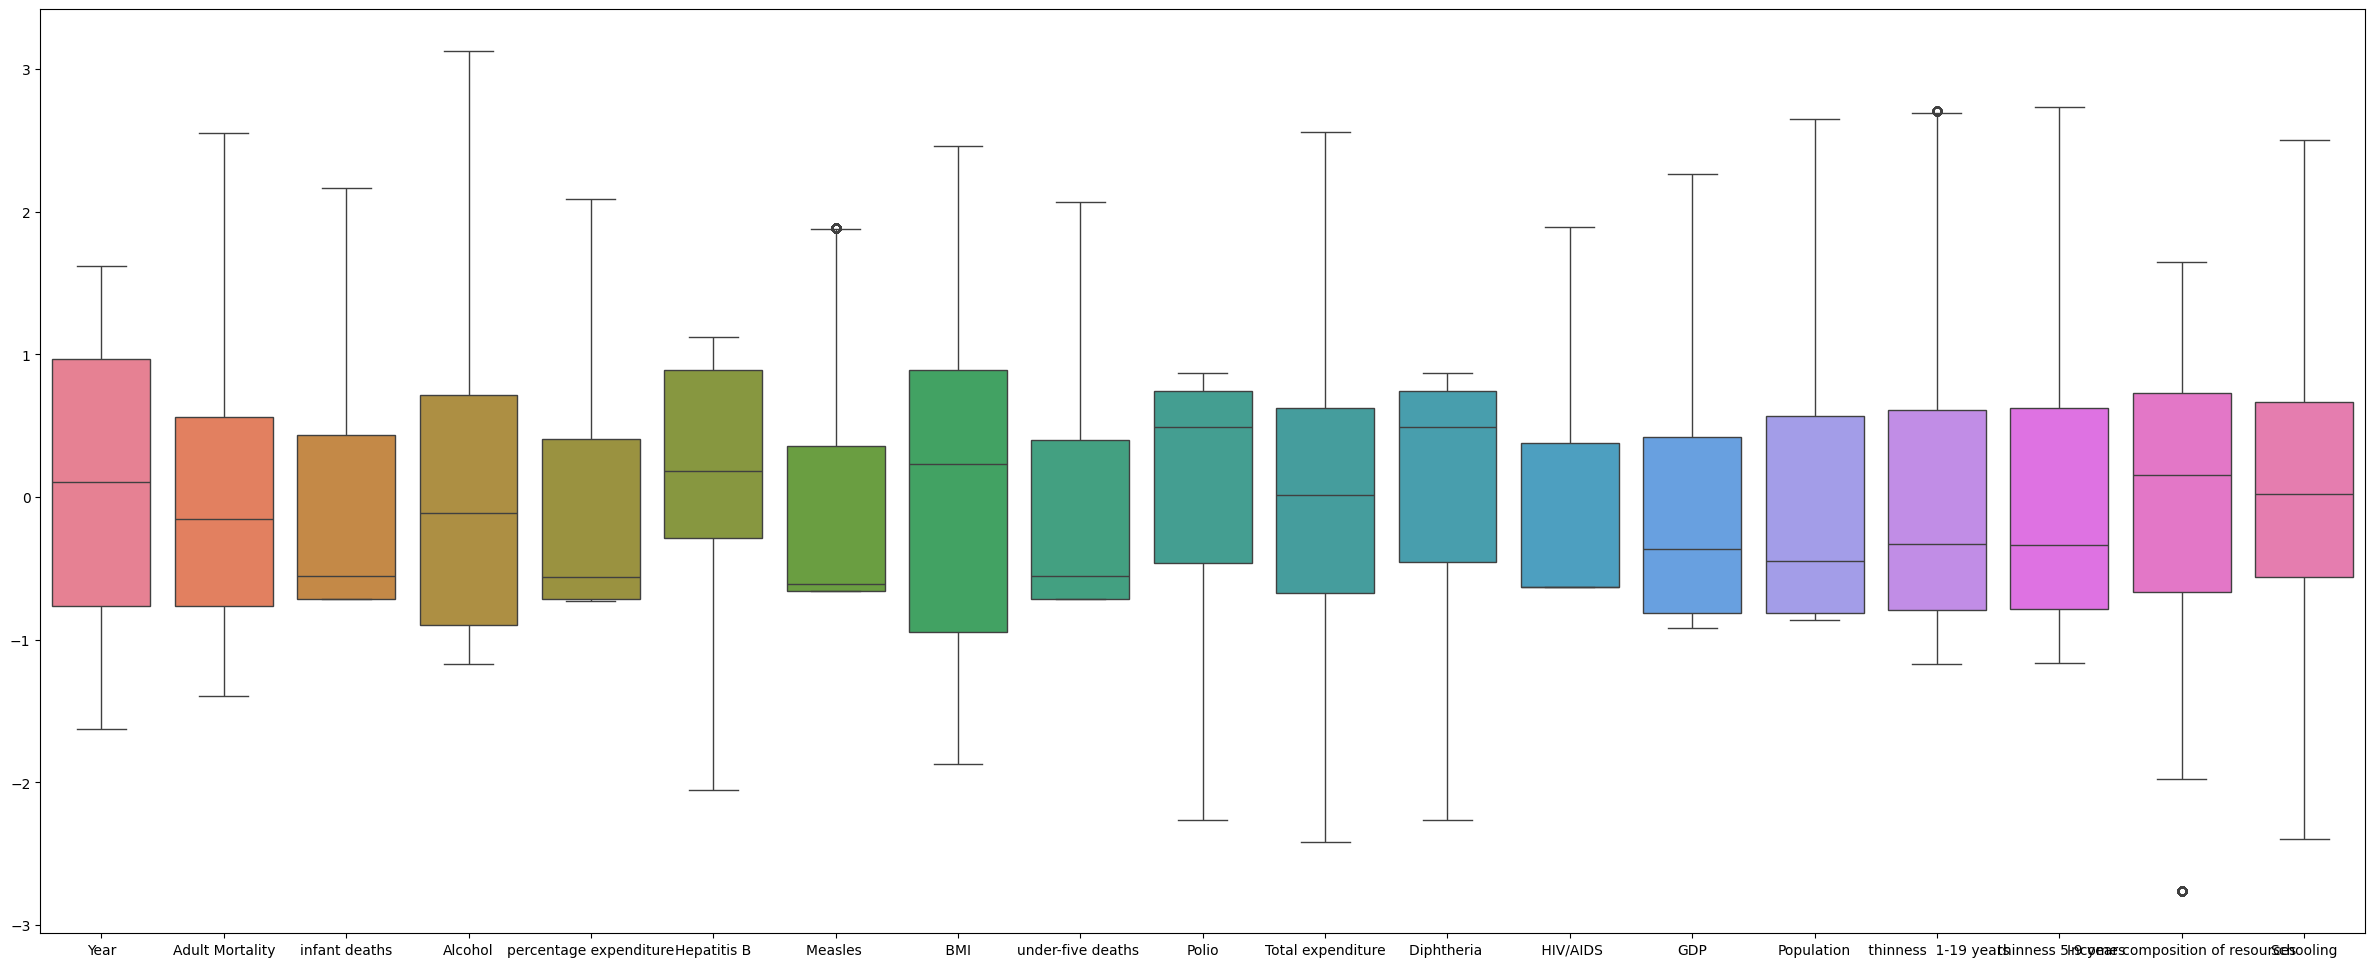
\includegraphics[width=\textwidth]{output.png}
    \caption{Boxplot distribution of standardized features}
\end{figure}

Many features show a wide range and several outliers, suggesting varied conditions across countries.

\subsection{Density and Histogram Plots}
We examined the overall distribution of the standardized variables using overlaid histograms and KDE plots.

\begin{figure}[H]
    \centering
    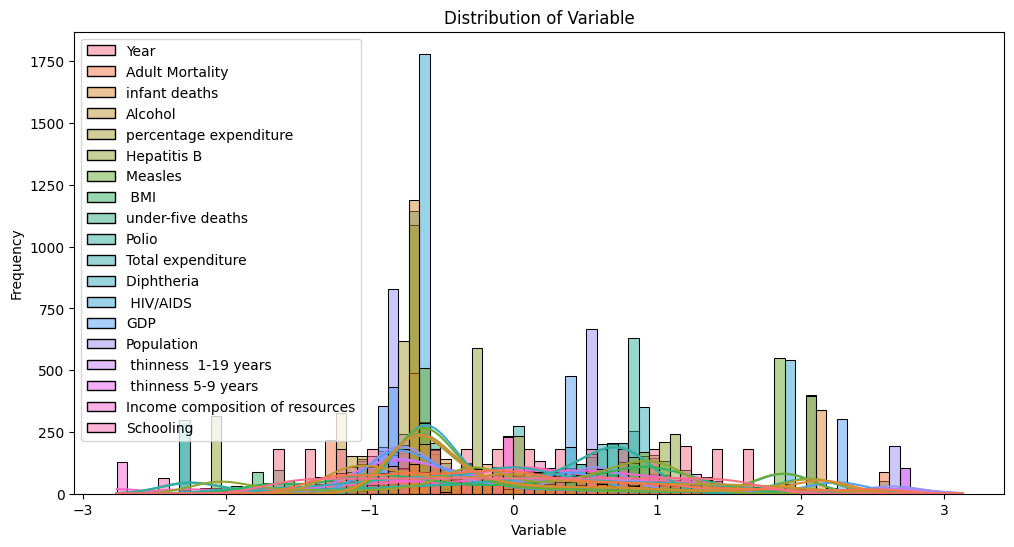
\includegraphics[width=0.85\textwidth]{output2.png}
    \caption{Distribution of variables (standardized)}
\end{figure}

Features like \texttt{GDP} and \texttt{Alcohol} show multimodal distributions, indicating country-specific clustering.

\subsection{Life Expectancy by Country Status}
We explored differences in life expectancy between developed and developing countries.

\begin{figure}[H]
    \centering
    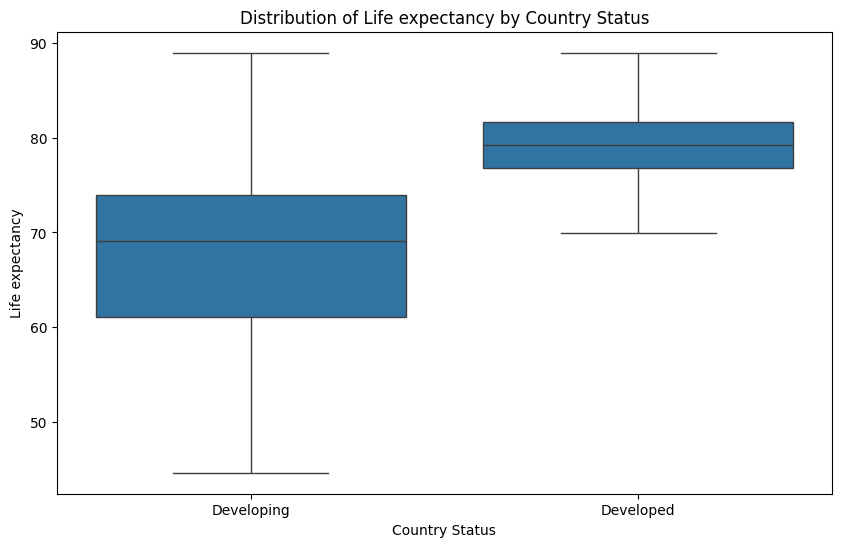
\includegraphics[width=0.7\textwidth]{output3.png}
    \caption{Life Expectancy by Country Status}
\end{figure}

Developed countries exhibit higher life expectancy with less variation, while developing countries show more spread and lower median.

\section{Statistical Hypothesis Testing}

\subsection{Test 1: Hepatitis B Vaccination by Country Status}
\begin{itemize}
    \item \textbf{Null Hypothesis:} There is no difference in Hepatitis B vaccination rates between developed and developing countries.
    \item \textbf{Alternative Hypothesis:} There is a significant difference.
\end{itemize}
A t-test revealed a significant difference ($p < 0.05$), with developed countries generally showing higher vaccination coverage.

\subsection{Test 2: Life Expectancy by Country Status}
\begin{itemize}
    \item \textbf{Null Hypothesis:} No difference in life expectancy.
    \item \textbf{Alternative Hypothesis:} There is a significant difference.
\end{itemize}
T-test confirmed the difference ($p < 0.01$), supporting the visual evidence from earlier.

\subsection{Test 3: Life Expectancy by Year}
Using ANOVA:
\begin{itemize}
    \item \textbf{Null Hypothesis:} Life expectancy is equal across years.
    \item \textbf{Alternative Hypothesis:} Life expectancy differs by year.
\end{itemize}
We found significant temporal variation in life expectancy.

\subsection{Test 4: Designed Hypothesis – BMI vs Life Expectancy}
We hypothesized that higher BMI may be positively correlated with life expectancy up to a point. Pearson correlation supported a mild positive correlation.

\subsection{Test 5: Designed Hypothesis – Schooling vs Life Expectancy}
Hypothesis: More years of schooling are associated with higher life expectancy. Correlation analysis showed strong positive relationship ($r > 0.6$).

\section{Correlation Analysis}
Correlation with target variable (Life expectancy):

\begin{itemize}
    \item \texttt{Schooling}, \texttt{Income composition of resources}, and \texttt{BMI} showed the highest positive correlation.
    \item \texttt{HIV/AIDS} and \texttt{Adult Mortality} showed the strongest negative correlation.
\end{itemize}

\section{Regression Modeling}

\subsection{Train-Test Split (No Overlap in Countries)}
We first split the data ensuring no country appeared in both train and test. Two models were trained:

\subsubsection*{With Country Column}
\begin{figure}[H]
    \centering
    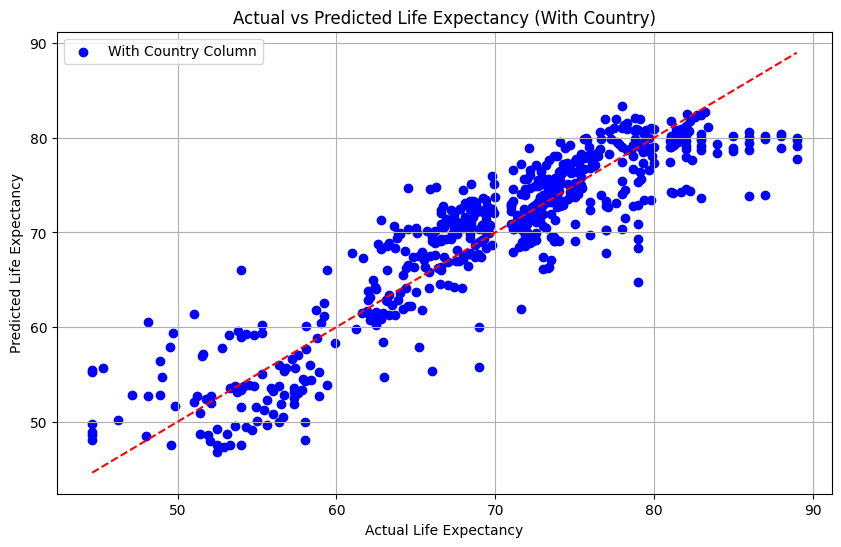
\includegraphics[width=0.7\textwidth]{output4.png}
    \caption{Predicted vs Actual Life Expectancy (With Country Column)}
\end{figure}

\subsubsection*{Without Country Column}
\begin{figure}[H]
    \centering
    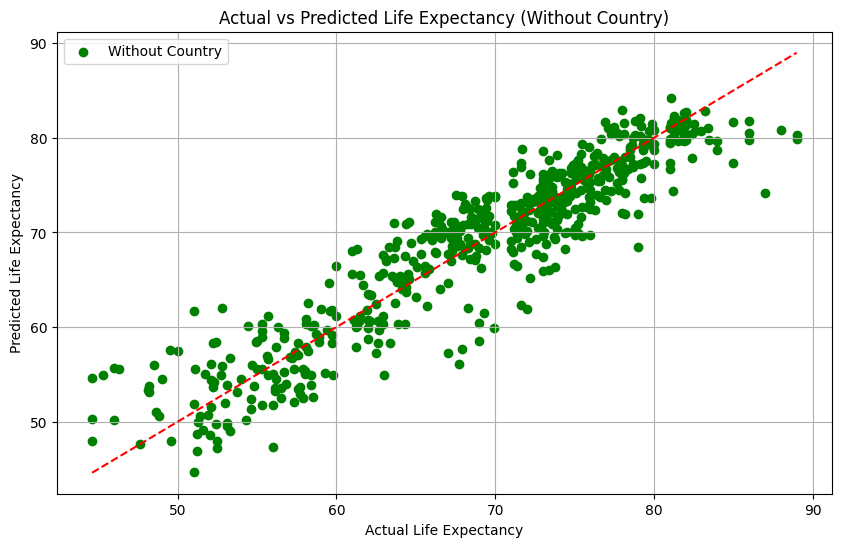
\includegraphics[width=0.7\textwidth]{output5.png}
    \caption{Predicted vs Actual Life Expectancy (Without Country Column)}
\end{figure}

\noindent The model without the country column generalizes better, avoiding overfitting to specific national patterns.

\subsection{Random Split and Re-evaluation}
Repeating the regression with a random split yielded improved test performance, showing slight overfitting in the first approach due to regional characteristics embedded in country names.

\subsection{Linear vs Lasso Regression}
We compared plain linear regression with L1 regularization:
\begin{itemize}
    \item Lasso dropped many irrelevant variables, making the model more interpretable.
    \item Variables with highest absolute weights matched those with high correlation values (e.g., \texttt{Schooling}, \texttt{Income composition}).
\end{itemize}

\section{Conclusion}
This analysis confirms that life expectancy is multifactorial, with education, healthcare spending, income distribution, and vaccination coverage being strong contributors. Statistical testing and correlation metrics helped validate these findings. Linear and Lasso regression models confirmed the influence of key variables. Avoiding country-based overlap during train-test split enhances generalizability, crucial for building robust predictive models.

\section*{References}
\begin{itemize}
    \item \url{https://www.kaggle.com/datasets/kumarajarshi/life-expectancy-who}
    \item \url{https://scikit-learn.org}
    \item \url{https://www.data-to-viz.com}
\end{itemize}

\end{document}
